\chapter{Diagnóstico} \label{cap:diagnostico}

Neste capítulo são apresentados o estado atual de trabalho da equipe, o estado desejado e as recomendações estabelecidas
a partir do diagnóstico realizado.

\section{Estado Atual}

% COLOCAR SOBRE O IL E O DESENV DE SOFTWARE AQUIIIIII 
A forma atual de trabalho da equipe de desenvolvimento pode ser caracterizada de acordo com os seguintes aspectos:

\begin{itemize}
  \item Utilização da metodologia ágil Scrum;
    \subitem Eventos: Reunião de Planejamento e Reunião de Revisão;
    \subitem Artefatos: Backlog do Produto e Backlog da Sprint.
  \item Duração da iteração de 1 semana;
  \item Processo imaturo;
  \item Processo não está devidamente formalizado;
  \item Processo pouco medido e controlado;
  \item Riscos tratados de forma reativa.
\end{itemize}

Já o SiGA pode ser caracterizado como um sistema que tem um alto número de defeitos decorrentes da implantação e um baixo número de testes.

Com o intuito de identificar as atividades empenhadas no desenvolvimento foi desenhado um esboço do processo atual 
que não é formalizado. Seu objetivo é estabelecer
as atividades de análise de requisitos, construção e implantação do incremento de software. Este processo pode ser visto na 
Figura \ref{fig:processo_atual} e o seu detalhamento encontra-se no Apêndice \ref{ap:processo_atual}.

\begin{figure}[!ht]
\centering
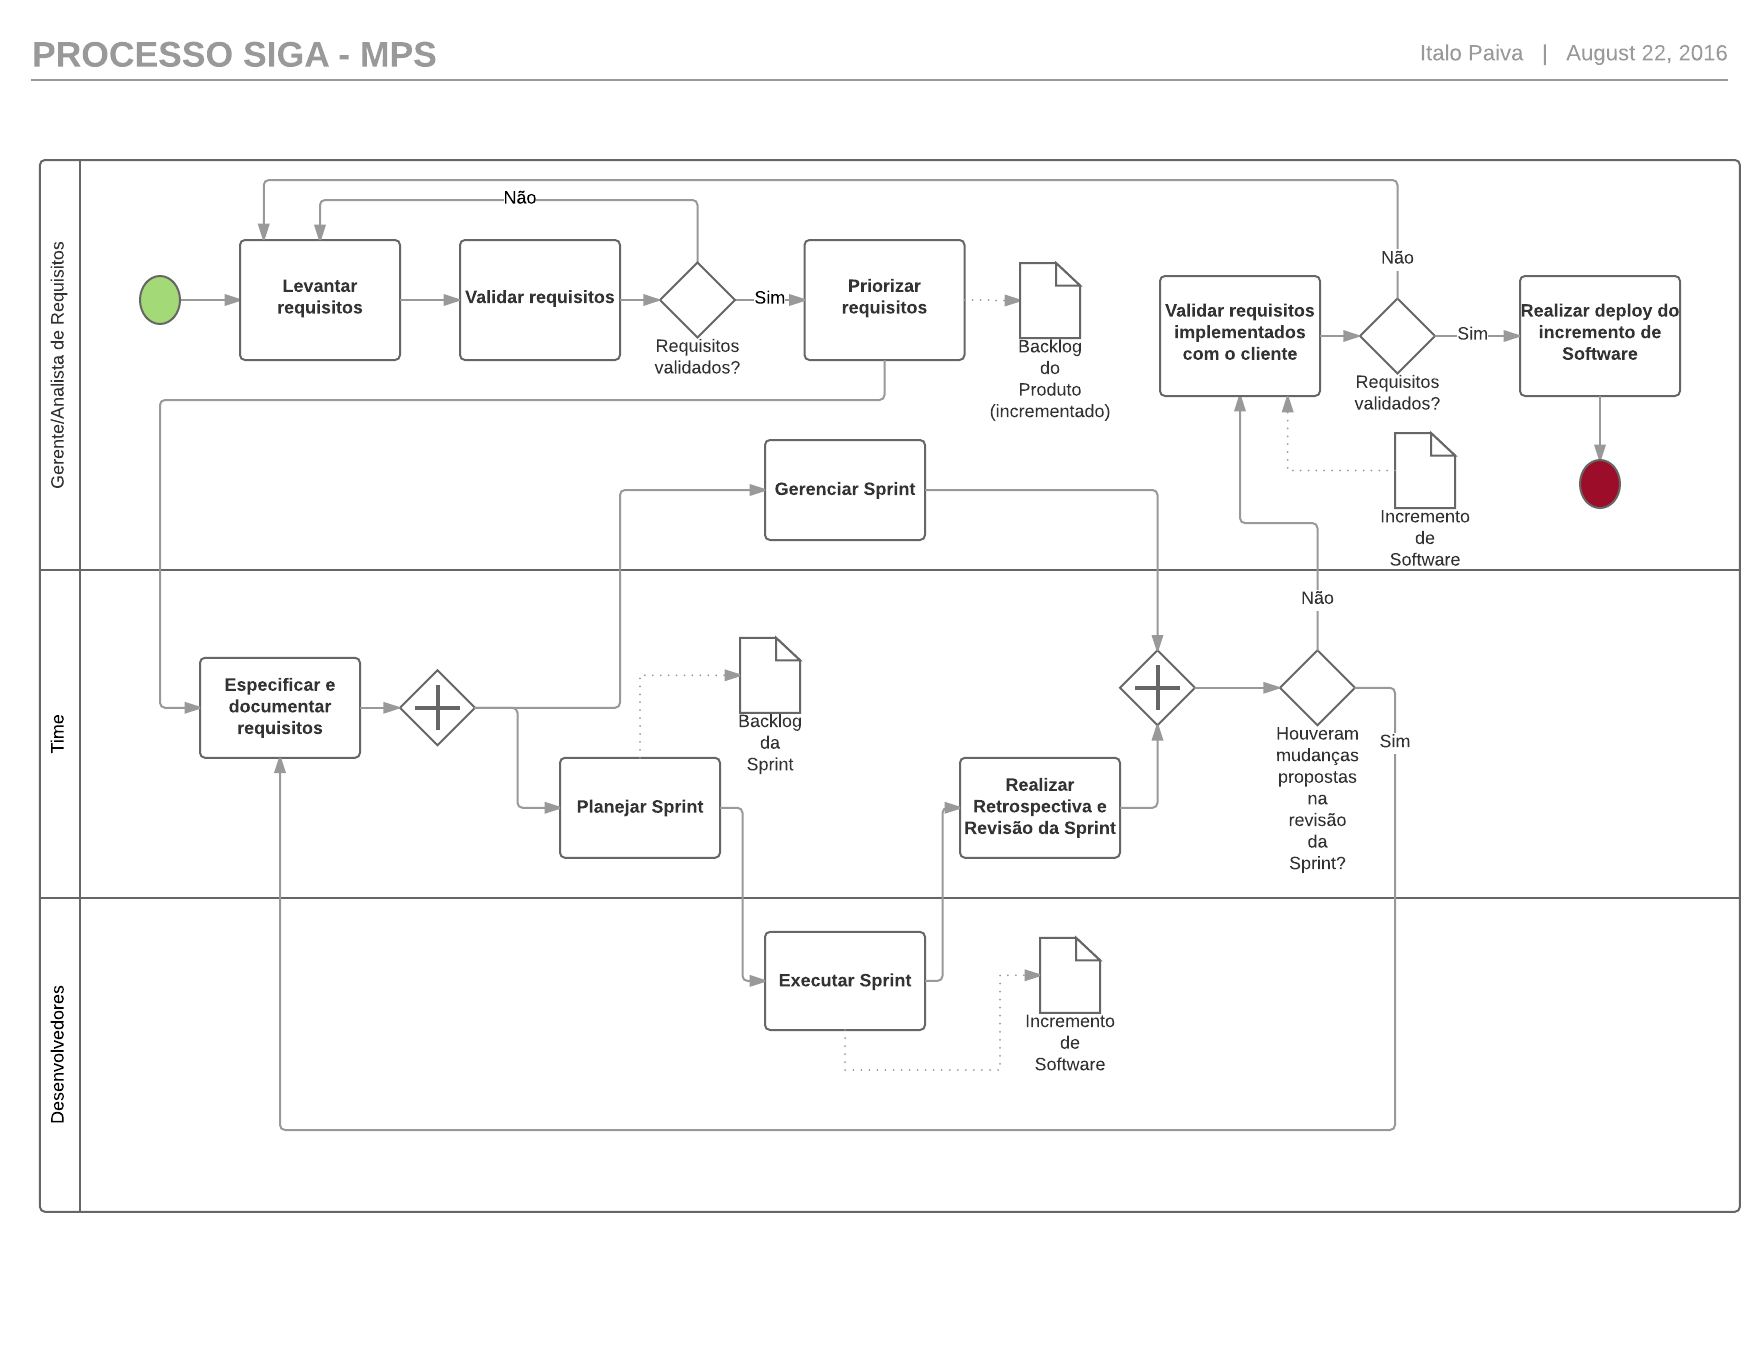
\includegraphics[scale=0.5]{figuras/processo_atual.png}
\caption{Processo Atual}
\label{fig:processo_atual}
\end{figure}


\subsection{Análise do processo}

A partir do processo descrito foi realizada uma análise para identificação dos problemas que impactam na qualidade do produto 
e na continuidade do trabalho. 

Analisando o processo é possível notar que há uma dificuldade nas atividades de testes e implementação. Foram percebidos
muitos defeitos decorrentes da implantação, ou seja, defeitos manifestados apenas em ambiente de produção. Além disso, 
os testes não são implementados em todas as iterações, embora o processo atual seja baseado em práticas ágeis não há a 
contínua garantia da qualidade. 

Foi percebido que a falta da definição de um processo e de um monitoramento acarreta em 
decisões técnicas e gerenciais reativas, assim como o tratamento a riscos. 

Na análise também foram identificadas algumas limitações relacionadas ao processo e ao produto. São elas: 

\begin{itemize}
  \item Ausência de boa ferramenta para realização de testes;
  \item Tempo de iteração fixo em 1 semana;
  \item Equipe pequena;
  \item Falta de acesso direto ao ambiente de produção;
\end{itemize}

\section{Estado Desejado}

Após a execução desse projeto é esperado que haja uma melhoria do processo apresentado na Figura \ref{fig:processo_atual}, 
considerando principalmente aspectos gerenciais e de qualidade. Também é esperado que este processo seja formalizado e utilizado
de fato pela equipe. Dessa forma, o estado desejado pode ser sumarizado nos seguintes itens:

\begin{itemize}
	\item Processo de desenvolvimento de software formalizado;
	\item Execução das atividades do processo padronizadas;
	\item Atividades de teste e implantação bem definidas;
	\item Diminuição dos defeitos decorrentes da implantação;
	\item Melhoria da suíte de testes;
	\item Processo minimamente medido e controlado.

\end{itemize}

	
\section{Recomendações}

A fim de alcançar o estado desejado foram estabelecidas algumas recomendações, são elas: 

\begin{itemize}
    \item Adicionar atividades de testes bem definidas no processo;
    \item Adicionar integração contínua no processo;
    \item Enfatizar o uso das práticas ágeis;
\end{itemize}
